\documentclass{beamer}
% PACKAGES --------------------------------------
\usepackage[utf8]{inputenc}
\usepackage[T1]{fontenc}

% GENERAL --------------------------------------

\usepackage{tikz} % Drawings
\usepackage{wrapfig} % Inline images
\usepackage{amsmath,amssymb,amsthm} % Advanced math
\usepackage{xcolor} % Colored text
\usepackage{hyperref} % Clickable TOC
\renewcommand{\baselinestretch}{1.2} % Line height
\usepackage{graphicx} % Graphics *but better*
\usepackage{adjustbox}
\usepackage{bookmark}
\usepackage{minted}
\usepackage{titling}

\setlength{\droptitle}{-8em}     % Eliminate the default vertical space
\addtolength{\droptitle}{-4pt}   % Only a guess. Use this for adjustment

% \graphicspath{{./img/}}

% \input{lib/glossary.tex} % Glossary
% \input{lib/nomenclature.tex} % Nomenclature/Symbolverzeichnis

% MACROS ----------------------------------------

% Displaystyle fractions
\newcommand\ddfrac[2]{\ensuremath{\frac{\displaystyle #1}{\displaystyle #2}}}

% TIKZ ------------------------------------
\usepackage{pgf,tikz,pgfplots}
\usepackage{mathrsfs}
\usetikzlibrary[patterns]
\pgfplotsset{compat=1.15}
\usetikzlibrary{arrows}
\newcommand{\degre}{\ensuremath{^\circ}}

% GERMAN --------------------------------------

\usepackage[ngerman]{babel} % german
\usepackage{csquotes}

% https://www.overleaf.com/learn/latex/Typesetting_quotations
% use \say{} to quote something
\usepackage[
    left = \glqq{},
    right = \grqq{},
    leftsub = \glq{},
    rightsub = \grq{}
]{dirtytalk} % Correct quotation marks

\newtheorem*{theorem}{Hypothese} % Rename
\addto\captionsngerman{%
    \renewcommand{\abstractname}{Vorwort}
}

% BIBLIOGRAPHY --------------------------------------

\usepackage[backend=biber,sorting=none]{biblatex}
\addbibresource{../bib/bib.bib}

% METADATA --------------------------------------

% SETUP --------------------------------------

\title{Objektrelationale Datenbanken - Handout}
\author{******** Nguyen}
\date{\today}



% DOCUMENT  --------------------------------------------------------

\begin{document}

\maketitle

\begin{frame}{Inhaltsverzeichnis}
  \setbeamertemplate{section in toc}[sections numbered]
  \tableofcontents[hideallsubsections]
\end{frame}

% All sections go into the ./sections folder
% Make sure to not include the .tex extension when including
\include{sections/einführung}
\section{Vergleich}

\begin{frame}
    \frametitle{Relational vs. Objektrelational}
    \pause
    \begin{columns}[T,onlytextwidth]
        \column{0.5\textwidth}
            \textbf{Relational}
            \pause
            \begin{itemize}
                \item Tabellarisch (in Reihen und Spalten) dargestellt \pause
                \item Primärschlüssel \pause
                \item Beziehungen zu anderen relationalen Datenbanken \pause
                \item Grundlegende Datentypen \pause
                \begin{itemize}
                    \item int, float/double, byte \pause
                    \item string, char \pause
                    \item bool, null \pause
                \end{itemize}
            \end{itemize}

        \column{0.5\textwidth}
            \textbf{Objektrelational}
            \pause
            \begin{itemize}
                \item Auch tabellarisch dargestellt
                \item Alles was im Relationalen möglich ist \pause
                \item Kann zusätzlich komplexere Datentypen nutzen \pause
                \begin{itemize}
                    \item Arrays (int[], string[] etc. \dots) \pause
                    \item Objekte (selber definierte etc. \dots) \pause
                    \item Objekte (selber definierte etc. \dots) \pause
                \end{itemize}
            \end{itemize}
    \end{columns}
\end{frame}

\begin{frame}
    \frametitle{Objektorientiert vs. Objektrelational}
    \pause
    \begin{columns}[T,onlytextwidth]
        \column{0.5\textwidth}
            \textbf{Objektorientiert}
            \pause
            \begin{itemize}
                \item In (Instanzen von) Objekten dargestellt, nicht Tabellen \pause
                \item $\rightarrow$ hat ebenfalls komplexe Datentypen \pause
                \item Geeignet für eine Codebase, welche auf OOP basiert \pause
            \end{itemize}

        \column{0.5\textwidth}
            \textbf{Objektrelational}
            \pause
            \begin{itemize}
                \item Tabellarisch
                \item Ebenfalls komplexe Datentypen
            \end{itemize}
    \end{columns}
\end{frame}

\begin{frame}
    \frametitle{Ähnlichkeit}

    \begin{table}
        \begin{small}
            \label{tab:OODBvsORDB}
            \begin{center}
                \begin{tabular}[c]{|r|l|}
                    \hline
                    \multicolumn{1}{|c|}{\textbf{Objektorientiert}} &
                    \multicolumn{1}{c|}{\textbf{(Objekt)relational}} \\
                    \hline
                    Klassen                   & Tabellen \\
                    Instanzen (eines Objekts) & Reihen in einer Tabelle \\
                    Attribute                 & Spalten \\
                    Objektreferenzen          & Fremdschlüssel/Beziehungen \\
                    \hline
                \end{tabular}
            \end{center}
            \caption{Parallelen zwischen objektorientiert und objektrelational}
        \end{small}
    \end{table}

\end{frame}

\section{Beispiele}

% Erwachsener/Kind
\begin{frame}
    \frametitle{Relationaler Datensatz mit Arrays?}

    \begin{columns}[T,onlytextwidth]
        \column{0.475\textwidth}
            \begin{table}
                \centering
                \begin{adjustbox}{width=\textwidth}
                    \small
                    \begin{tabular}[c]{|c|c|c|c|c}

                        \hline

                        \multicolumn{1}{|c|}{\textbf{id}} &
                        \multicolumn{1}{c|}{\textbf{name}} &
                        \multicolumn{1}{c|}{\textbf{vorname}} &
                        \multicolumn{1}{c|}{\textbf{alter}} &
                        \multicolumn{1}{c}{\dots} \\

                        \multicolumn{1}{|c|}{\textit{int}} &
                        \multicolumn{1}{c|}{\textit{String}} &
                        \multicolumn{1}{c|}{\textit{String}} &
                        \multicolumn{1}{c|}{\textit{int}} &
                        \multicolumn{1}{c}{\dots} \\

                        \hline

                        0  & Mustermann  & Max    & 27             & \dots \\
                        1  & Mustermann  & Marie  & 26             & \dots \\
                        2  & Fröhlich    & Nico   & 18             & \dots \\
                        3  & Hammer      & Niko   & \textit{null}  & \dots \\
                        $\vdots$ & $\vdots$ & $\vdots$ & $\vdots$ &

                    \end{tabular}
                \end{adjustbox}
                \caption{Datensatz \say{Erwachsene} als relationale Datenbank}
                \label{tab:erwachsene1}
            \end{table}

        \pause

        \column{0.475\textwidth}
        \begin{table}
            \centering
            \begin{adjustbox}{width=\textwidth}
                \small
                \begin{tabular}[c]{|c|c|c|c|c}

                    \hline

                    \multicolumn{1}{|c|}{\textbf{id}} &
                    \multicolumn{1}{c|}{\textbf{name}} &
                    \multicolumn{1}{c|}{\textbf{vorname}} &
                    \multicolumn{1}{c|}{\textbf{alter}} &
                    \multicolumn{1}{c}{\dots} \\

                    \multicolumn{1}{|c|}{\textit{int}} &
                    \multicolumn{1}{c|}{\textit{String}} &
                    \multicolumn{1}{c|}{\textit{String}} &
                    \multicolumn{1}{c|}{\textit{int}} &
                    \multicolumn{1}{c}{\dots} \\

                    \hline

                    0  & Mustermann  & John   & 8   & \dots \\
                    1  & Mustermann  & Jan    & 3   & \dots \\
                    2  & Mustermann  & Phil   & 5   & \dots \\
                    3  & Hammer      & Paul   & 1   & \dots \\
                    $\vdots$ & $\vdots$ & $\vdots$ & $\vdots$ &

                \end{tabular}
            \end{adjustbox}
            \caption{Datensatz \say{Kinder} als relationale Datenbank}
            \label{tab:kinder1}
        \end{table}

    \end{columns}
\end{frame}

% Arrays
\begin{frame}
    \frametitle{Relationaler Datensatz mit Arrays?}

    \begin{table}
        \centering
        \begin{adjustbox}{width=\textwidth}
            \small
            \begin{tabular}[c]{|c|c|c|c|c|c}

                \hline

                \multicolumn{1}{|c|}{\textbf{id}} &
                \multicolumn{1}{c|}{\textbf{name}} &
                \multicolumn{1}{c|}{\textbf{vorname}} &
                \multicolumn{1}{c|}{\textbf{alter}} &
                \multicolumn{1}{c|}{\textbf{kinder}} &
                \multicolumn{1}{c}{\dots} \\

                \multicolumn{1}{|c|}{\textit{int}} &
                \multicolumn{1}{c|}{\textit{String}} &
                \multicolumn{1}{c|}{\textit{String}} &
                \multicolumn{1}{c|}{\textit{int}} &
                \multicolumn{1}{c|}{\alert{int[]?}} &
                \multicolumn{1}{c}{\dots} \\

                \hline

                0  & Mustermann  & Max    & 27            & \alert{[0,1,2]?}  & \dots \\
                1  & Mustermann  & Marie  & 26            & \alert{[0]?}      & \dots \\
                2  & Fröhlich    & Nico   & 18            & \textit{null}     & \dots \\
                3  & Hammer      & Niko   & \textit{null} & \alert{[3]?}       & \dots \\
                $\vdots$ & $\vdots$ & $\vdots$ & $\vdots$ & $\vdots$ &

            \end{tabular}
        \end{adjustbox}
        \caption{Datensatz \say{Erwachsene} als objektrelationale Datenbank}
        \label{tab:erwachsene2}
    \end{table}

\end{frame}

\begin{frame}
    \frametitle{Relationaler Datensatz mit Objekten?}
    % minted kinda doesnt want to compile in the beamer environment so i have to use this bad alternative which makes me sad. verbatim doesnt work either for some stupid reason.
    \begin{figure}
        \begin{small}
            \begin{center}
                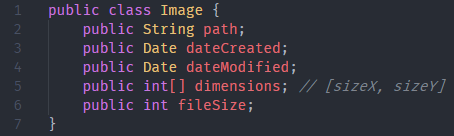
\includegraphics[width=0.95\textwidth]{img/ClassExample.png}
            \end{center}
            \caption{Beispiel einer \say{Image} Klasse}
            \label{fig:image}
        \end{small}
    \end{figure}
\end{frame}

\begin{frame}
    \frametitle{Relationaler Datensatz mit Objekten?}

    \begin{table}
        \centering
        \begin{adjustbox}{width=\textwidth}
            \small
            \begin{tabular}[c]{|c|c|c|c|c|c}

                \hline

                \multicolumn{1}{|c|}{\textbf{id}} &
                \multicolumn{1}{c|}{\textbf{name}} &
                \multicolumn{1}{c|}{\textbf{vorname}} &
                \multicolumn{1}{c|}{\textbf{alter}} &
                \multicolumn{1}{c|}{\textbf{portrait}} &
                \multicolumn{1}{c}{\dots} \\

                \multicolumn{1}{|c|}{\textit{int}} &
                \multicolumn{1}{c|}{\textit{String}} &
                \multicolumn{1}{c|}{\textit{String}} &
                \multicolumn{1}{c|}{\textit{int}} &
                \multicolumn{1}{c|}{\alert{Image}} &
                \multicolumn{1}{c}{\dots} \\

                \hline

                0  & Mustermann  & Max    & 27             & \alert{<Instanz>}      & \dots \\
                1  & Mustermann  & Marie  & 26             & \alert{<Instanz>}      & \dots \\
                2  & Fröhlich    & Nico   & 18             & \textit{null}  & \dots \\
                3  & Hammer      & Niko   & \textit{null}  & \alert{<Instanz>}     & \dots \\
                $\vdots$ & $\vdots$ & $\vdots$ & $\vdots$ & $\vdots$ &

            \end{tabular}
        \end{adjustbox}
        \caption{\say{Erwachsene}\dots mit Bildern?}
        \label{tab:erwachsene3}
    \end{table}

\end{frame}

\section{Fazit}

\begin{frame}
    \frametitle{Fazit}

    \metroset{block=fill}

    \begin{block}{Eine objektrelationale Datenbank ist\dots}
        \pause
        wie als hätten relationale und objektorientierte Datenbanken ein Kind gemacht!
    \end{block}

\end{frame}

\begin{frame}[standout]
    Fragen?
\end{frame}

\appendix

\begin{frame}
    \frametitle{Quellen}
    \nocite{*}
    \printbibliography
\end{frame}


% \include{sections/sources}
\end{document}
